\setlength{\abovedisplayskip}{2pt}
\setlength{\belowdisplayskip}{2pt}
\section{Monte Carlo Study}
\label{sec:monte_carlo}

In this section we will first talk about topics that concern users of Bayesian methods.  We will introduce the concept of convergence in the Bayesian context and discuss the choice of a meaningful predistribution. Then we will present the results of our Monte Carlo study with a focus on different prior distributions.

\subsection{Convergence}

In most cases, we calculate Bayesian models by taking random samples from the underlying distribution. As shown in the previous chapter we use Markov chain Monte Carlo methods like the Metropolis hastings algorithm, because they converge to the equilibrium of the model. Once we have achieved convergence the following draws will be drawn from the underlying distribution. \\
Since bayesian estimation methods are computationally intensive, there is a great demand for methods that reliably determine convergence.\\
As a first step, the first half (or quarter) of draws should be discarded to mitigate the the influence of the initial parameters and allow the algorithm time to converge. In the next step we test wether the algorithm is converged and extend the burn-in period if not.
Since parameter draws with a higher posterior value are accepted more frequentuently, the chain flucuates around the posterior mode once it has converged. Therefore a graphical analysis of the draws is a frequently used technique to monitor convergence.\\
Also, parts of the chain can be compared with each other using statistical methods. The idea is that if the algorithm did converge, parameters are drawn from the same distribution and therefor should be sufficiently similar.For example, the Gekwek`s Diagnostic compares the parameter mean of the first 10\% and 50\% of the draws while taking the autocorrelation of draws into account (\cite{geweke1992}).\\
However, \cite{brooks1998} argue that it is not possible to determine convergence with a single chain. As with many other iterative optimizations the optimizer can get stuck in a region with a low density for a long time.Therefor, one should start with several highly dispersed starting values to detect false convergence with a higher probability. In a well-known paper \cite{gelman1992} instead proposes to compare the variance of several parallel chains.
We follow their approach and calculate the Gelman-Rubin Convergence Diagnostic to capture convergence in our simulation study.\\
To do this, we start several chains M$\geq$2 with N draws (after the burn-in period). 
For every paramter of our model, we calculate the chain variance $s_m^2$ as $\frac{1}{N-1}\sum_{n=1}^{N} (\theta_m^{(n)}-\overline{\theta}_m )^2$ using $\overline{\theta}_m=\frac{1}{N} \sum_{n=1}^{N} \theta_m^{(n)}$.\\
We derive the average within-chain-variance W by averaging over all M chains.\\
$$W=\frac{1}{M} \sum_{m=1}^{M} s_m^2 $$ 
And calculate the between sequence variance B/N as:
$$B/N=\frac{1}{M-1} \sum_{m=1}^{M} (\overline{\theta}_m-\overline{\theta} )^2 $$
using the average draw of all chains $\overline{\theta}=\frac{1}{M} \sum_{m=1}^{M} \theta_m$.
Brooks and Gelman derive an estmate of the total variance as a weighted sum of with-in chain variance and between chain variance.
$$\widehat{var}^+ (\theta \mid y)=\frac{N-1}{N}W+\frac{1}{N}B$$
This estimate will be unbiased when we reached convergence and will overestimate the variance when we start with widely distributed inital values (\cite{brooks1998}).
If we take our sampling uncertainty about our posterior mean $\overline{\theta} $ into account we derive the posterior Variance estimate $\widehat{V}$ as $\widehat{var}^+ (\theta \mid y) +\frac{B}{MN}$ 
.\\
The second part of the equation is often neglected as N is large enough in most circumstances (for example Stan uses the simplified version).
Finally, the potential scale reduction statistic is defined by the equation:
$$\widehat{R}=\sqrt{\frac{\widehat{V}}{W}}$$
If the algorithm converged, then the whole variance follows from the underlying distribution. The within-chain variance is large compared to the between-chain variance and $ \widehat{R}$ is close to 1.\\
$\widehat{R}$ is much bigger if the estimate of the total variance is poor. Or if there are big differences between the different chains, because they did not converge to the same value.  In both cases, we should increase the number of iterations. In general, a scale reduction factor below 1.1 strongly suggests overall convergence, while a scale reduction factor below 1.2 weakly suggests.\cite{brooks1998}


\subsection{Stan Configurations}
We use the open-source package Stan for the calculation of  Bayesian hierarchical models. Stan is an C\texttt{++} package with its programming language for coding probability models.  Bayesian models can be fit with bayesian and maximum likelihood methods. We accessed Stan via the interface Pystan in the programming language Python. Because Stan compiles our model into C\texttt{++} code, we can realize fast run times using a standard laptop.\\
Stan uses the Nuts-Sampling algorithm based on the Hamilton Monte Carlo (HMC) with the advantage  over other Markov Chain Monte Carlo methods that it produces distant candidate draws, hereby incresasing effective sample size and convergence of the algorithm.
On the other hand, the efficiency of HMC is highly sensitive to tuning parameters leapfrog stepsize $\epsilon$ and number of leapfrog steps, L. \cite{neal2011}. % write sentence about Hamiton Monte Carlo leapfrog and steps form neal
The No-U-turn sampler by \cite{hoffman2014} opened the use of the HMC to many other areas by automatically setting optimal parameter values for leapfrog stepsize and leapfrog steps. \\
%Stan uses the hamilton Monte Carlo modified around the no-uturn sampler and we use it exclusively in our Monte Carlo study. The first part of burn-in perior is used to tune the parameters of the model.
%For every (current) trajectory Stan measures how 
%Stan measures how the (current) trajectory would lead the MCMC to new areas. If this trajectory would lead it far from the posterior mean, it will report a high divergence value, and we risk wandering around areas with a low posterior value for a long time. By setting a higher target acceptance, we (indirectly) decrease the stepsize, because variables with higher posterior values will be accepted more often. Consequently, we limit the sampled region of the posterior.
%We might want to use a higher acceptance rate of $\delta$ if we have to happen a high convergence in our draws. For every draw, 
%Depending on the convergence results of our Monte Carlo runs (and friendly recommendations of Stan) we change the (target) acceptance rate $\delta$.\\
%By setting $\delta$, we can change the (expected) probability that a draw with a smaller posterior value lowe, then the value of the current draw is kept. The default value of the target acceptance rate is 0.8, which happens to be around the optimal value under some normality assumptions. Roberts, Gelman, and Gilks (1997). \cite{roberts1997b}
%In Stan this target acceptance rate influences the stepsize of the Hamilton Monte Carlo algorithm. A higher stepsize increase the range of possible candidate draws around the current draw $\theta_i$. Therefore if we have a high stepsize (and we are currently around the posterior mean), many draws with a low posterior value will be proposed and subsequently rejected. If the step size is too small, we will accept many draws, but most of them will be in the small distance to the posterior mean. Therefore we will need a long time to discover the full posterior distribution. \cite{stan2018}

We can further increase the efficency of the Markov Chain Monte Carlo algorithm by starting with initial values close the posterior mean. Because this value is unknown ex-ante a common strategy is to solve for the posterior mean with a numerical optimizer (e.g., Stan uses the quasi-newton algorithms LBFGS as a default). Then we sample intial values for our M chains from a fat tailed distribution like the t-distribution around the value (\cite{brooks1998}).
As seen in figure \ref{fig:convergence}, Hamilton Monte Carlo encountered no problems to finding the posterior mode of our simple models. Therefor we use the default option of stan - Initial values are drawn from the UNI[-2,2]. If parameters are constrained, they are transformed into the unconstrained space before. For example, intial values of the standard deviation are drawn from the intervall $[e^{-2},e^2]$.   




\subsection{Monte Carlo Preparations}
% introduce model
In our Monte Carlo study we ask ourselves how the calculation of bayesian hierarchical models reacts to different prior distributions on our hyperparameters.
We analyze the performance in respect to the random slope model with group characteristics.

\begin{align}
  y_i &= \alpha+ x_i^\prime \beta_{j[i]} + \epsilon_i \,,\\
  \beta_{j[i]} &= \gamma_0 + u_j^\prime \gamma + \eta_j \,,
\end{align}

Varying slope models are widely used in political science, educational research and psychology. For example, \cite{snijders2012} reference such a model to test the effects of social status($x_i$) on the left-right positioning ($y_i$) of individuals. The impact of social status on political affiliation $\beta_{j[i]}$ are allowed to be different for individuals of different countries J. They depend on the level of inequality in this country ($u_j$)  and random effects $\eta_j$.\\
If $u_j$ is demeaned, we can interpreted $\gamma_0$  as the constant effect of inidividual characteristic, while $\gamma_1$ indicates how group-characteristics shape the effects of individual characteristics.\\
In our simulation study we analyze the performance of bayesian models by estimating both parameters. We fix the group characteriscs $u_j$ and individual characteristcs $x_i$, but draw new realizations of  $\eta$, and $\epsilon$ in every simulation run. \\

We tested two different data generating processes in our analysis: \\

1) we use non-centered characteristics $u_j$ and $x_i$ as\\

$x_i \sim N(5,0.3)$ , $\epsilon \sim N(0,\sigma_y) $ , $u_j \sim N(5,0.3)$ , $\eta \sim N(0,1) $ , $\eta \sim N(0,\sigma_b)$\\
and fixed parameters $\alpha=1$, $\gamma_0=1$ , $\gamma_1=1$ , $\sigma_b=\sigma_y=1$\\

2) we use centered characteristics $U_j$ and $x_i$ with more variation: \\ 

$x_i \sim N(0,3)$ ,  $\epsilon \sim N(0,\sigma_y) $ , $u_j \sim N(0,3)$ , $\eta \sim N(0,1) $ , $\eta \sim N(0,\sigma_b)$\\
and fixed parameters $\alpha=1$, $\gamma_0=1$ , $\gamma_1=1$ , $\sigma_b=\sigma_y=1$ \\

% choosing the right prior
The selection of a meaningful prior distribution is the best known feature of bayesian statistics and a frequent source of criticism. In some situations we can incorporate external knowledge for determining prior distributions. For example, many macroeconomic studies estimate the discount factor $\beta$ between 0.93 and 1.01 with the average around 0.99 for most countries (e.g. \cite{rumler2007}).
In other situations the information situation is unclear. While it is desired that our prior distribution will have direct conseqences on our estimates, it is not the desirable that the prior completely dominates the new information from the data ("let the data speak").\\
An extra difficulty comes from the fact that the strength of a prior can only be determined in the context of likelihood. It is therefore a common strategy to select prior distributions according to the data basis (\cite{gelman2017prior}). 
Often different prior designs are tested and selected based on their comparability to the data (\cite{leeper2017clearing}).
If the size of the effect is unknown in advance it also makes sense to normalize the input data. For example, the impact of wealth on risk aversion will change depending on the currency unit in which wealth is nominated. It was found that scaling of the input data also influences the efficiency of the algorithm (\cite{gelman2008weakly}). \\
In our Monte Carlo study we test the effect of informative, weakly informative and uninformative prior distribuitons on our bayesian estimations.
The idea is to start with an informative prior distribution around the true mean of our parameters $\gamma_0=\gamma_1=1$. Then we move the prior distribution one unit to the right - giving the prior a upward distortion.
Next, we turn our prior distribution into a weakly informative one by increasing the standard distribution of priors from 1 to 3.
We also try a less shifted prior distribution and a uniform prior distribution. See Table \ref{tab:prior_table} for an overview of the prior distributions we have chosen. In the following we will often use the short name of the prior distributions for better readability.\\
In all our simulations we use a Half-Cauchy (0,5) prior for the standard deviations of the innovations $\eta$ and $\epsilon$, repectively. With an median of 5 and a fat tail, Half-Cauchy (0,5)  is an weak prior with negligible influence on the results.
By default we calculate our models with 10 groups and 200 individuals per group, but we also look at the effect of reducing the size and number of groups. All the simulations that do not converge are sorted out in the analysis.
However, we require a total of 300 simulations for each model. Depending on the convergence results we increase the number of burn-in draws or change the stan parameters. Our standard stan parametrization can be found in the appendix  in Table \ref{tab:default_1} and Table \ref{tab:default_2}.



\begin{table}[!ht]
\begin{center}
\begin{tabular}{l l l l l l}
Prior specification & Short-Name for Model & $\gamma_0$ & $\gamma_1$ & $\sigma_y$,$\sigma_\beta$\\
\hline
True, strong priors &  True & $\normal{1,1}$ & $\normal{1,1} $ & $C^+(0, 5)$\\
Wrong, strong priors & Wrong  &$\normal{2,1}$ & $\normal{2,1}$ & $C^+(0, 5)$\\
Wrong, weak priors &  Weakwrong  & $\normal{2,3}$ &$ \normal{2,3}$ & $C^+(0, 5)$\\
Slightly wrong, weak priors &  Weakslighltywrong & $ \normal{1.2,3}$ &$\normal{1.2,3}$ & $C^+(0, 5)$\\
Uniform prior & Uniform &$\mathcal{U(-\infty,1)}$ & $\mathcal{U(-\infty,1)}$ & $C^+(0, 5)$\\
\end{tabular}
\end{center}
\caption{The prior distributions of our hyperparameters $\gamma_0$, $\gamma_1$, $\sigma_\beta$ and  $\sigma_y$}
\label{tab:prior_table}
\end{table}


\subsection{Monte Carlo Results}

We assess the performance of bayesian method using four different criteria.
First, we calculate the average posterior mean of all of our sample runs. We use this metric to identify bias in our estimations. 
Second, we calculate [$5\text{\%}$, $95\text{\%}$] intervalls of the posterior mean estimates. Ex ante, we can assign a probility of 90\% to the event, that our parameter will fall in this range. We can the intervall to test how stable our estimations are in respect to changing input data. 
Third, we calculate average [$5\text{\%}$, $95\text{\%}$] posterior intervalls. This metric gives us an estimate of the average uncertainty in the calculation of the parameters.
Forth we calculate [$2.5\text{\%}$, $97.5\text{\%}$] intervalls for our parameter draws in every simulation run. Then we count how many times the true parameter falls  inside of the intervall. If the true parameters falls into this range more than 95\% of the times our confidence intercalls are conservative. Otherwise they are too optimistic.This intervall - called credible set in the bayesian literature - is used by Researchers to determine the statistical significance of a parameter in Bayesian statistics. If a value does not fall within this interval, we would have rejected it in our analysis. \cite{koop2003}.\\
In our Monte Carlo study we use the posterior mean as the point estimate models of our model parameters. Practioners also use the mode or median of the posterior. Because posterior distributions are not symmetric by nature the estimates will be different. However, the results were similar when we tried the median instead of the mean table \ref{tab:median}.\\

As can be seen in Table  \ref{tab:bias_first}, our Bayesian Methods performed far worst for our first data-generating-process. We severly underestimate $\gamma_0$, while overestimating $\gamma_1$.
A reason for this is that the parameters of the group model are interdependent.A bias in one of the parameters worsens the calculation of all other parameters.  Therefore we expect a good fit for all parameters or none of them. Our group characteristics are not centered around zero, so an underestimation of $\gamma_0$  can be offset by an increase in $\gamma_1$. See graph \ref{fig:wrong_prior_dgp1} for the effect of a wrong prior on the parameter estimation.
In accordance with \cite{gelman2008weakly}, scaling has a big impact on the efficiency of our estimations as well. 
It took far longer to fit the model to our first data-generating process  and Hamilton Monte Carlo showed slower convergence (see \ref{fig:convergence}). Thus our first DGP shows anecdotal evidence that problems with fitting a model often arise because of wrong parametrization/modeling.
\\
Consequently, we directed our further analysis to the second data generating process.
First, we calculate the average posterior mean for $\gamma_0$,$\gamma_1$, $\sigma_b $ and $\sigma_y$ in all simulation runs.
As can be seen in Table\ref{tab:bias_second} our estimate of $\sigma_y$ is very close to the true value regardless of prior selection or number of groups. This is not suprising since we work with large sample sizes in our model. 
The average mean of the intercept parameter $\gamma_0$ is close to true parameter as well. Although we observe that a wrong prior pulls the average estimate in its direction.
The slope parameter $\gamma_1$ was biased upwards in all of our simulation runs and the bias increases with a wrong prior. Interestingly, we decrease the bias by roughly 2/3 if we increase the standard deviation of our (wrong) prior distribution from 1 to 3. \\
We overestimated the standard deviation $\sigma_b$ in all our configurations. This is not surprising since we only have 5-10 groups in our Monte Carlo and use a weakly informative prior distribution. An increase of $\sigma_b$ is accompanied by a worst fit of all parameter. The exception to this rule is the model with a uniform prior. Our estimates of the hyperparameters $\gamma_0$ and $\gamma_1$ are less biased, while the standard deviation $\sigma_b$ increase greatly.\\
 
Surprisingly, the positive bias of $\gamma_0$ and $\gamma_1$ drops when we decrease the number of individuals per group from 200 to 100 (see Table \ref{tab:means}). In the model with the wrong prior we calculate $\gamma_1$  as average 1.11 instead of 1.19. 
By reducing the sample size the likelihood becomes less important compared to the prior. Therefore, a smaller group size should result in worse calculations and an increase in bias. Alarmingly the average variance of $\sigma_b$ rises, which was connected with a worst fit in previous runs. So we take a closer look at the relationship between the posterior mean estimates $\eta$ (of group 1) and the calculations of $\gamma_1$ for a model with a wrong prior. 
We fit a (gaussian) density to the posterior means of $\eta$ and $\gamma_1$ using the seaborn. In the following we always refer to an estimate of the density when we talk about a density.
Then we plot both against each other in \ref{fig:various sample size}. \\
If we use 200 individuals and 10 groups (a) we can see that the wrong prior distorts the calculations. However, the deviations are similar across simulations. And the deviations centre around some point with a positive bias in $\gamma_0$ and a negative bias in $\eta$.
If we use only 100 individuals per groups (b) our estimations become unstable. Many posterior means assemble around a new centre with a negative bias in $\gamma_1$ and a positive bias in $\eta_1$. The average bias drops, because the bias in the old and new centre partly cancel each other out. Since this is only due to a greater instability, we exclude the simulations with only 100 individuals from further analysis.\\
If we decrease the number of groups J to 5 and keep 200 individual (c),we increase the variance in our estimates.  But we do not make the calculations unstable.
See also \ref{fig:posterior_wrong_gamma0} and \ref{fig:posterior_wrong_gamma1} for the plottet posterior distributions. 

% continue from here
\begin{figure}[h!]
  \centering
  \begin{subfigure}[b]{0.3\linewidth}
    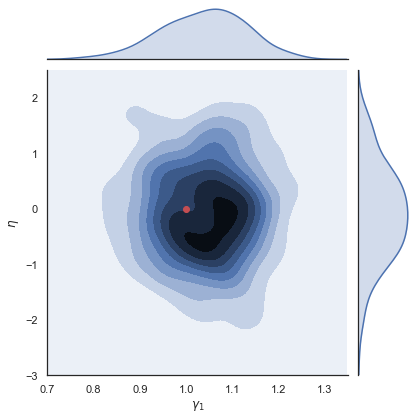
\includegraphics[width=\linewidth]{graphics/jointplot_gamma1eta_big}
    \caption{ N=200, J=10}
  \end{subfigure}
  \begin{subfigure}[b]{0.3\linewidth}
    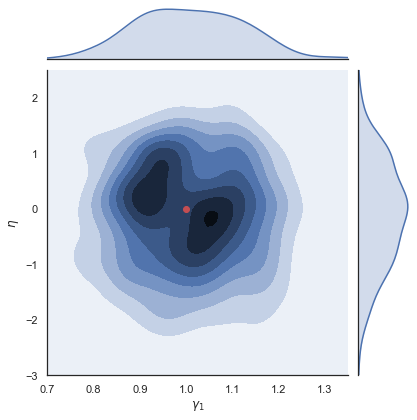
\includegraphics[width=\linewidth]{graphics/jointplot_gamma1eta_small}
    \caption{N=100, J=10}
  \end{subfigure}
  \begin{subfigure}[b]{0.3\linewidth}
    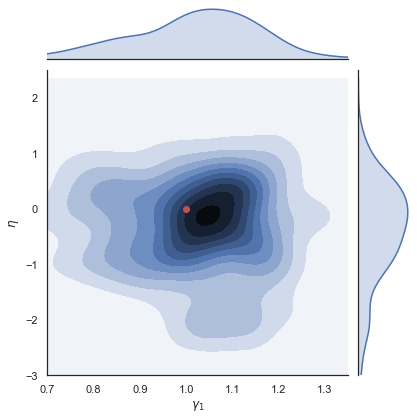
\includegraphics[width=\linewidth]{graphics/jointplot_gamma1eta_smallJ}
    \caption{ N=200, J=5}
  \end{subfigure}
  \caption{Joint-Density of posterior mean estimates of $\gamma_1$ and $\eta$ in a model with a wrong specified prior;
  Red dot denotes the expected value}
  \label{fig:various sample size}
\end{figure}


Next, we compare the posterior means of our simulation runs. In figure \ref{fig: gamma0 and gamma1}, we plotted the posterior densities of $\gamma_0$ and $\gamma_1$ of our 300 simulation runs. Our estimate of $\gamma_0$ shows a high variability. Since new realizations of $\eta$ are drawn in each simulation, the intercept $\gamma_0$ will be strongly influenced by them. By working with a higher number of groups J, we decrease the variability through the law of large numbers(see Figure \ref{fig:gamma0_posterior} (a) vs (c)).
The estimation of $\gamma_1$  changes very little in every simulation run. Our group characteristics stay constant and are informative in predicting the impact of individual characteristcs $\beta$. 
The calculation of $\gamma_1$ therefore changes little even if we use different prior distributions. As can be seen in Table \ref{tab:means} the 5\% percentile of $\gamma_1$ is between 0.83-0.85 for 10 groups and 0.73-0.78 for 5 groups.
The 5\% percentile of $\gamma_0$ is between 0.46-0.69 and 0.24-0.76, repectively.\\
In graph \ref{fig:gamma0_posterior} we compare the posterior densities of $\gamma_0$ in a model with a wrong prior (a) and a uniform prior (b). We can observe that the wrong prior increase the bias by shifting the posterior to the right. The uniform prior does increase the variability in the posteriors modes and results in thicker tails.\\
In \ref{fig:weak_uni} we plotted a density of the mean estimates of $\gamma_0$ when using a weakwrong prior and a uniform prior. The weak, but wrong prior raises the bias of our estimate, but raises the curvature. That means we have more accurate mean estimates in more of our scenarios, while getting slighlty worst on average. The effect is stronger if we use only a small number of groups J=5. If we increase the number of groups, the likelihood begins to dominate the posterior and the estimates approach each other. \\
As can be seen in Table \ref{tab:means} the weak, but wrong prior do improve the estimation of $\gamma_0$. The weak priors lead to higher 5\% lower estimates and lower 95\% higher estimates of the posterior means. The effect is stronger when working with a smaller number of groups J and when the prior mode is closer to the true value.\\
We can see the observe the same effect for the calculation of $\gamma_1$. However, the effects are much smaller.\\

\begin{figure}[h!]
  \centering
  \begin{subfigure}[b]{0.4\linewidth}
    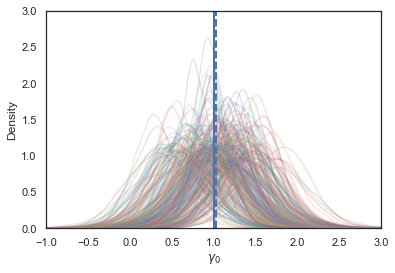
\includegraphics[width=\linewidth]{graphics/posterior_plot_gamma0}
    \caption{True Prior, N=100, J=10}
  \end{subfigure}
  \begin{subfigure}[b]{0.4\linewidth}
    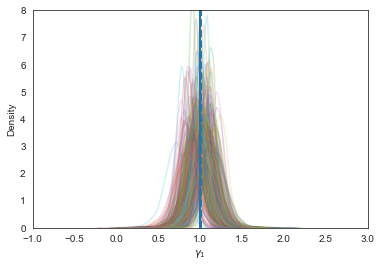
\includegraphics[width=\linewidth]{graphics/posterior_plot_gamma1}
    \caption{True Prior, N=200, J=10}
  \end{subfigure}
  \caption{Posterior densities  of $\gamma_0, \gamma_1$, Blue line: True Value, Dotted line: Average Estimate}
  \label{fig: gamma0 and gamma1}
\end{figure}

\begin{figure}[h!]
  \centering
  \begin{subfigure}[b]{0.4\linewidth}
    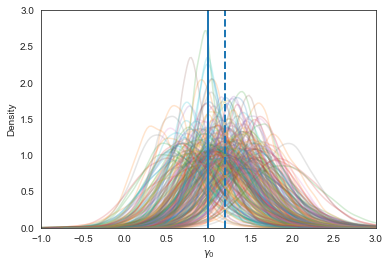
\includegraphics[width=\linewidth]{graphics/posterior_plot_gamma0_wrong}
    \caption{Wrong Prior, N=100, J=10}
  \end{subfigure}
  \begin{subfigure}[b]{0.4\linewidth}
    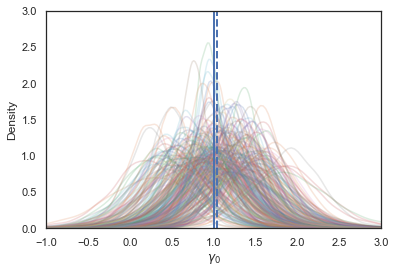
\includegraphics[width=\linewidth]{graphics/posterior_plot_gamma0_uni}
    \caption{Uni Prior, N=200, J=10}
  \end{subfigure}
  \caption{Posterior densities of $\gamma_0$, Blue line: True Value, Dotted line: Average Estimate}
  \label{fig:gamma0_posterior}
\end{figure}

\begin{figure}[h!]
  \centering
  \begin{subfigure}[b]{0.4\linewidth}
    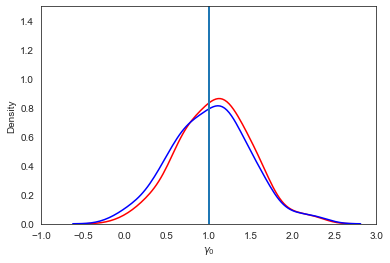
\includegraphics[width=\linewidth]{graphics/mean_plot_gamma0_unib_weakwrongr}
    \caption{Weakwrong(red) vs Uniform(blue)}
  \end{subfigure}
  \begin{subfigure}[b]{0.4\linewidth}
    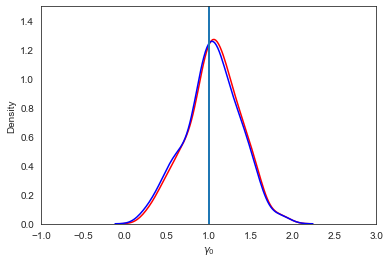
\includegraphics[width=\linewidth]{graphics/mean_plot_gamma0_unib_weakwrongr2}
    \caption{Weakwrong(red) vs Uniform(blue)}
  \end{subfigure}
  \caption{Posterior mean densities of $\gamma_0$, J=5 (left) and J=10 (right)}
  \label{fig:weak_uni}
\end{figure}


In Table \ref{tab:quantiles} we compare the average [0.05,0.95] posterior percentiles of our model parameters $\gamma_0$ and $\gamma_1$. 
This metric gives us an estimate of how large the average uncertainty is when calculating the parameters. We can observe that a wrong prior increases the variation in our estimates and shifts the range to the right. 
In accordance with our intuition the priors with a higher standard deviation lead to wider credible sets of our estimations. Consequently, the model with the uniform prior has the widest credible set for both parameters. In accordance with our previous results, the percentiles are greater for $\gamma_0$ than for $\gamma_1$ and explode if we decrease the number of classes to 5.\\
Next we check how often the true parameter falls into the [0.05,0.95] confidence intervall (Table \ref{tab:coverage}) of our posterior distribution. Suprisingly, the ratio of runs is very high (around 97\%) and stays high for all priors.
We tested other quantiles as well and came up with similar results. Therfor our simulation study speaks in favor of the often talked about claim that bayesian modelling is a more conservative approach to other likelihood based estimation methods.  (e.g.\cite{stegmueller2013}). Even using wrong and strong prior distribution does not lead to rejecting the right parameters more often, because the credible sets adjust to a higher difference of prior and likelihood.

\subsection{Conclusion and Limitations of our work}

In our simulation study we found out that many observations are needed to calculate a model with varying slope and group characteristics. Furthemore, normalization of input data can increase the accuracy and efficiency of calculations and non-convergence is often a signal for a bad fit. We have confirmed that informative prior distributions are often a better choice than uninformative prior distributions and are particularly useful for small sample sizes. However, since a false prior lead to bias, they should be sufficiently weak no prior knowledge is available.\\
On the other hand there are also some limitations of our simulation study. We have performed our analysis with smaller sample size than usual in the most other studies. \cite{stegmueller2013} worked with 500 individuals and 1000 simulations, while we limited ourselves to 300 simulations and 200 individuals. More indiduals increase the complexity of likelihood and thus multiply the required computational resources. These models could not be analyzed with an ordinary laptop (a single run took between 1-5 min). Our intervalls are much wider as a results. \\
Furthermore, we have not worked with different class sizes or put the results of our calculations in context with other statistical methods. These points are addressed in the following application part.




